\chapter{Building Simulation Programs}
\label{cha:building-simulation-programs}

\section{Overview}

As it was already mentioned, an {\opp} model physically consists of
the following parts:

\begin{itemize}
  \item{NED language\index{ned!files} topology description(s). These
      are files with the \ttt{.ned} extension.}
  \item{Message definitions\index{message definitions}, in files
      with \ttt{.msg} extension.}
  \item{Simple modules implementations and other C++ code, in \ttt{.cc}
        files (or \ttt{.cpp}, on Windows)}
\end{itemize}


To build an executable simulation program,
you first need to translate the MSG files\index{msg!files}
into C++, using the message compiler (\ttt{opp\_msgc}).
After this step, the process is the same as building any C/C++
program from source: all C++ sources need to be compiled into object files
(\ttt{.o} files (using gcc on Mac, Linux) or mingw on Windows), or \ttt{.obj} (using MSVC on Windows)),
and all object files need to be linked with the necessary libraries to get
an executable or shared library.

\begin{note}
Compiling NED files directly to C++ classes is no longer supported in
{\opp} 4.0. NED files are always dynamically loaded.
\end{note}

File names for libraries differ for Unix/Linux and for Windows,
and also different for static and shared libraries.
Let us suppose you have a library called Tkenv.
If you are compiling with gcc or mingw, the file name for the static library
would be something like \ttt{libopptkenv[d].a},
and the shared library would be called \ttt{libopptkenv[d].so}.
(libopptkenvd.so would be used for the debug version while libopptkenv.so
is for the release build.) The Windows version of the static library would
be \ttt{libopptkenv.a}, and the DLL would be named \ttt{libopptkenv.dll}.

\begin{note}
With MSVC, the corresponding filenames will be \ttt{opptkenv.lib} and \ttt{opptkenv.dll}.
On Mac OS X, shared libraries have the \ttt{.dylib} extension instead of \ttt{.so}.
\end{note}

In {\opp} 4.0 we recommend to use shared libraries whenever it is possible.
You'll need to link with the following libraries:

\begin{itemize}
  \item{The simulation kernel and class library\index{simulation!kernel},
    called \textit{oppsim} (file \ttt{liboppsim.[so|dll|dylib]} etc).}
  \item{User interfaces. The common part of all user interfaces is
    the \textit{oppenvir} library (file \texttt{liboppenvir.[so|dll|dylib]}, etc),
    and the specific user interfaces are \textit{opptkenv} and \textit{oppcmdenv}
    (\ttt{libopptkenv.[so|dll|dylib]}, \ttt{liboppcmdenv.[so|dll|dylib]}, etc).
    You have to link with \textit{oppenvir}, plus \textit{opptkenv} or
    \textit{oppcmdenv} or both.}
\end{itemize}

Luckily, you do not have to worry about the above details, because
automatic tools like \ttt{opp\_makemake} will take care of the hard
part for you.

The following figure gives an overview of the process of building
and running simulation programs.

\begin{figure}[htbp]
  \begin{center}
%%XXX    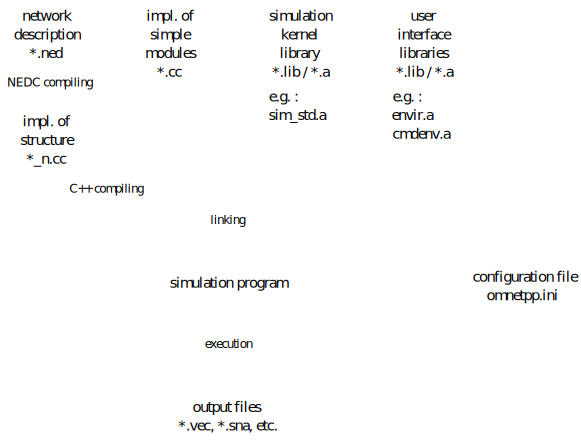
\includegraphics[width=5.992in, height=4.519in]{figures/build}
    \includegraphics{figures/workflow}
    \caption{Building and running simulation}
  \end{center}
\end{figure}


This section discusses how to use the simulation system on the
following platforms:
\begin{itemize}
  \item{Unix (Linux/Mac OS X) with gcc}
  \item{Windows with the included MinGW}
\end{itemize}


\section{Using gcc}

This section applies to using {\opp} on Linux, Solaris, Mac OS X, FreeBSD and
other Unix derivatives, and also to MinGW on Windows.

Here in the manual we can give you a rough overview only.
The \ttt{doc/} directory of your {\opp} installation contains
\ttt{Readme.}\textit{<platform>} files that provide
up-to-date, more detailed and more precise platform specific
instructions.


\subsection{Installation}

The installation process depends on what distribution you take
(source, precompiled RPM, etc.) and it may change from release
to release, so it is better to refer to the readme files.
If you compile from source, you can expect the usual GNU
procedure: \ttt{./configure} followed by \ttt{make}.


\subsection{Building simulation models}

The \fprog{opp\_makemake} script can automatically generate a
\texttt{Makefile} for your simulation program, based on the source files
in the current directory or directory tree.
\fprog{opp\_makemake} has several options; \ttt{opp\_makemake -h}
displays a help text.

Once you have the source files (\ttt{*.ned}, \ttt{*.msg}, \ttt{*.cc},
\ttt{*.h}) in a directory, change there and type:

\begin{verbatim}
% opp_makemake
\end{verbatim}

This will create a file named \texttt{Makefile}\index{Makefile}. Thus if you
simply type \fprog{make}, your simulation program should build. The name of
the executable will be the same as the name of the directory
containing the files.


The freshly generated \texttt{Makefile} contains
dependencies\index{Makefile!dependencies}, but you can later
regenerate the dependencies by typing \fprog[make]{make depend}.
The warnings during the dependency generation process can
be safely ignored.

In addition to the simulation executable, the \texttt{Makefile}
contains other targets, too. Here is a list of important ones:

\begin{longtable}{|l|p{8cm}|}
\hline
\tabheadcol
\tbf{Target} & \tbf{Action}\\\hline
all & The default target is to build the simulation executable\\\hline
depend & Adds (or refreshes) dependencies in the \texttt{Makefile}\\\hline
clean &  Deletes all files that were produced by the make process\\\hline
\end{longtable}

If you already had a \texttt{Makefile} in that directory, \fprog{opp\_makemake}
will refuse to overwrite it. You can force overwriting the old \texttt{Makefile}
with the -f option:

\begin{verbatim}
% opp_makemake -f
\end{verbatim}

If you have problems, check the path definitions (locations of include
files and libraries etc.) in the configure.in script\index{configure script}
and correct them if necessary. Then re-run configure for the changes
to take effect.

You can specify the user interface (Cmdenv/Tkenv) with the -u option
(with no -u, both Cmdenv and Tkenv is linked in by default (this is the
recommended configuration)):

\begin{verbatim}
% opp_makemake -u Tkenv
\end{verbatim}

or:

\begin{verbatim}
% opp_makemake -u Cmdenv
\end{verbatim}

The name of the output file\index{output!file} is set with the -o
option (the default is the name of the directory):

\begin{verbatim}
% opp_makemake -o aloha
\end{verbatim}

If some of your source files are generated from other files (for
example, you use generated NED files), write your make rules
into a file called \ttt{makefrag}. When you run \fprog{opp\_makemake}, it
will automatically insert \ttt{makefrag} into the resulting \texttt{makefile}.
With the -i option, you can also name other files to be included into the
\texttt{Makefile}.


\subsection{Multi-directory models}

In the case of a large project, your source files may be spread across
several directories and your project may generate more than one executable
file (i.e. several shared libraries, examples etc.).

First identify each source directory tree in your project. A good rule of
thumb is that each source directory tree will generate a single output file
(i.e. shared/static library or executable file). A single project may contain
several source directory trees. A source directory tree needs
a \texttt{Makefile} in its root, but source files may be placed anywhere
in the tree. To specify that the generated \texttt{Makefile} should look into all
subfolders use the \texttt{opp\_makemake --deep} option. Make will descend into
subdirectories recursively and discover all \texttt{.cc}, \texttt{.h} and \texttt{.msg}
files. If you need to exclude a specific directory, use the \texttt{-X excude/dir/path}
option.

Your source directory tree may contain parts which need their own hand written \texttt{Makefile}.
This can happen if you include source files from an other non {\opp} project. To
include this handwritten \texttt{Makefile} into the build proecess first exclude that part
of the source tree from the deep file discovery by using the \texttt{-X project/with/own/makefile}
and use the \texttt{--subdir project/with/own/makefile} option to instruct \texttt{opp\_makamake}
to call the handwritten \texttt{Makefile} directly. (You may specify additional dependencies by
adding them to the \texttt{makefrag} file in the root of the source tree. This file will be
automatically included in your generated \texttt{Makefile} before all targets.)

If your source tree contains several subdirectories (maybe several levels deep) it is
annoying that you should specify relative paths for your header files in your \texttt{.cc} files
or you should specify the include path explicitly by the \texttt{-I includepath} option.
\texttt{opp\_makemake} has a default automatic include path discovery which adds all necessary
include directories in the current source tree to the compiler command line. The only requirement is
that your \texttt{\#include} statements must unambigously specify the name of the header file.
(i.e. if you have two \texttt{common.h} files one in subdir1 and the other in subdir2 specify
\texttt{\#include "subdir1/common.h"} instead of \texttt{\#include "common.h"}. If you want to
include a directory which is outside of your source directory tree you always must specify it with
the \texttt{-I external/include/dir} option.

\begin{note}
You may turn off the include autodiscovery mechanism with the \texttt{--no-deep-includes} option.
\end{note}

The next step is to decide whether you want to use static linking\index{static linking},
shared or run-time loaded (shared) libraries\index{shared libraries}. (We strongly
recommend to use shared libraries.) By default the makefile will create an executable
file from your source tree. Use \texttt{--make-so} to create shared libraries
or \texttt{--make-lib} to build static libraries instead. The \texttt{--nolink}
option completely avoids the linking step (useful for top level makefiles which do
not link themselves, but call the makefiles in the source directories).

Once you decided the type of your output file, you may specify additional external library
dependencies. Use \texttt{-Ldir} to specify external library directory and \texttt{-llibrary}
to specify the name of the external dependecy.

The \texttt{--recurse} option enables recursive make: when you build the simulation, make
will descend into the subdirectories and runs make in them too.
By default, \texttt{--recurse} decends into all subdirectories; the -X directory option
can be used to make it ignore certain subdirectories. This option is especially useful
for top level makefiles.

Once you have created your makefiles with \texttt{opp\_makemake} in every source directory tree
you will need a toplevel makefile. The toplevel makefile usually calls only the makefiles
recursively in the source directory trees.

You can control the build order by adding dependencies among subdirectories
into the \ttt{makefrag} file.

\subsection{A multi-directory example}

For a complex example of using opp\_makemake, we will check how to create
the makefiles for the mobility-framework. First take a look at the
project's directory structure and find the directories that should be used as
source trees:

\begin{verbatim}
mobility-framework
    bitmaps
    contrib <-- source tree (build libmfcontrib.so from this dir)
    core <-- source tree (build libmfcore.so from this dir)
    docs
    network
    template
    testSuite <-- source tree (build testSuite executable from this dir)
\end{verbatim}

Additionally there are dependencies between these output files: \texttt{mfcontrib}
requires \texttt{mfcore} and \texttt{testSuite} requires both \texttt{mfcore}
and \texttt{mfcontrib}.

First create the makefile for the core directory (build a shared lib from all .cc files
found in the core subtree and name it 'mfcore'):

\begin{verbatim}
% cd core && opp_makemake -f --deep --make-so -o mfcore -O out
\end{verbatim}

The contrib directory is depending on \texttt{mfcore} so we use the -L and -l options
to specify the library we should link with. Note that we must also add
the include directories manually from the core source tree, because autodiscovery works only
in the same source tree:
\begin{verbatim}
% cd contrib && opp_makemake -f --deep --make-so -o mfcontrib -O out -I../core/basicModules -I../core/utils -L../out/$(CONFIGNAME)/core -lmfcore
\end{verbatim}

The testSuite will be created as an executable file which depends on both
\texttt{mfcontrib} and \texttt{mfcore}.
\begin{verbatim}
% cd testSuite && opp_makemake -f --deep -o testSuite -O out -I../core/utils -I../core/basicModules \\
    -I../contrib/utils  -I../contrib/applLayer -L../out/$(CONFIGNAME)/contrib -lmfcontrib
\end{verbatim}

Now the last step is to create a top-level makefile in the root of the project that
calls the previously created makefiles in the correct order. We will use the
--nolink option, exclude every subdirectory from the bild (-X.) and explicitly call
the above makefiles (-d dirname).
\begin{verbatim}
% opp_makemake -f --nolink -O out -d testSuite -d core -d contrib -X.
\end{verbatim}

Finally we have to specify the dependencies between the above directories. Add the lines below to the makefrag file
in the prkeject directory root.
\begin{verbatim}
contrib_dir: core_dir
testSuite_dir: contrib_dir
\end{verbatim}

\subsection{Static vs shared {\opp} system libraries}

Default linking uses shared libraries\index{shared libraries}. One
reason you would want static linking is that debugging\index{debugging}
the {\opp} class library may be easier with static libraries.
Another reason might be that you want to run the executable on
another machine without having to worry about setting the
\fvar{LD\_LIBRARY\_PATH} variable (which should contain the name
of the directory where the {\opp} shared libraries are).

If you want static linking\index{static linking}, you must
recompile the {\opp} class library. Use

\begin{verbatim}
make clean
make SHARED_LIBS=no
\end{verbatim}

in the root of your {\opp} installation.

%%TODO --- include only in OMNEST build
\section{Using Windows and Microsoft Visual C++}

There are only slight differences to the way Microsoft Visual C++
is handled. The main differences are:
\begin{itemize}
  \item{You should use \ttt{opp\_nmakemake} instead of \ttt{opp\_makemake}}
  \item{The generated makefile will be called \ttt{Makefile.vc} by default.}
  \item{Use \ttt{makefrag.vc} instead of \ttt{makefrag}.}
  \item{\ttt{nmake} is used instead of \ttt{make}.}
  \item{The build process is started by \ttt{nmake -f Makefile.vc} instead of \ttt{make}.}
\end{itemize}

\subsection{Installation}

It is easiest to start with the binary installer version.
It contains all necessary software and precompiled
libraries except MSVC\index{MSVC}, and you can get a
working system up and running very fast.

Later you'll probably want to build the source yourself.
Reasons for that might be to compile the libraries
with different flags, to debug into them, or to recompile
with support for additional packages (e.g. Akaroa, MPI).
Compilation should be painless (it takes a single
\ttt{nmake -f Makefile.vc} command) after you get the different
component directories right in \ttt{configuser.vc}.


Some caveats:

\begin{itemize}

 \item \tbf{changed compiler settings}. Changes since {\opp} 2.2:
   You'll need exception handling and RTTI turned ON, and
   stack size set to as low as 64K.
   See the readme file for rationale and more hints.

\end{itemize}



%%% Local Variables:
%%% mode: latex
%%% TeX-master: "usman"
%%% End:
